%%% Local Variables:
%%% coding: utf-8
%%% mode: latex
%%% TeX-master: t
%%% End:
%
% -----------------------------------------------------------------------------
%  Kochbuch - Moppels Rezeptsammlung                          % vim:sw=2:ts=2
% -----------------------------------------------------------------------------
%
% general document setup
\documentclass[
	10pt,
	a4paper,
	titlepage,
	oneside]{book}
  \usepackage{kochbuch}
  \hypersetup{
    pdftitle={Moppels Rezeptsammlung},
    pdfsubject={Inspiriert von verschiedenen Sterneköchen},
    pdfauthor={Lutz Moppert},
    pdfkeywords = {Stichwort1, Stichwort2 ...} ,
    pdfcreator  = {pdflatex},
    }
%
% -----------------------------------------------------------------------------
%  Document colors
%
% Colors for title page
\colorlet{SubjectColor}{ForestGreen}
\colorlet{TitleColor}{ForestGreen}
\colorlet{SubtitleColor}{ForestGreen}
\colorlet{AuthorColor}{ForestGreen}
\colorlet{DateColor}{ForestGreen}

% Color for Recipes
\colorlet{PartColor}{NavyBlue}
\colorlet{ChapterColor}{OliveGreen}
\colorlet{RecipeColor}{OliveGreen}
\colorlet{IngredientColor}{OliveGreen}
\colorlet{LetterColor}{OliveGreen}

% Layout Colors
\colorlet{PageNumberColor}{MidnightBlue}
\colorlet{PageHeadFootColor}{MidnightBlue}
\colorlet{IndexHeadingColor}{MidnightBlue}

% Set general font for document
\usepackage[sfdefault,light]{roboto}

%
%  Ende der Preambel
% -----------------------------------------------------------------------------
%
\begin{document}
%
% -----------------------------------------------------------------------------
%  Titelseite
%
\frontmatter
\begin{titlepage}
\begin{center}
	\vspace*{4cm}
	\Huge{\textbf{\textcolor{TitleColor}{Cooking}}} \\[15pt]
	\LARGE{\textcolor{SubjectColor}{How to do it, and survive}} \\
% ----------------------------------------------------------------
	\vspace{1.5cm}
	\large{\textcolor{AuthorColor}{Author}}\\[5pt]
	\Large{\textbf{\textcolor{AuthorColor}{Author Name}}} \\
	\vfill
 % ----------------------------------------------------------------
	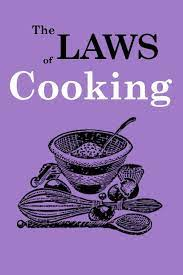
\includegraphics[width=0.35\textwidth]{images/title.jpg}\\[5pt]
	\vspace{1cm}
	{\textcolor{DateColor}{January 2022}}
\end{center}
\end{titlepage}

\newpage

% Table of contents
\tableofcontents
%
% -----------------------------------------------------------------------------
%  Main part
%
\mainmatter

\part{Gerichte}

\category[images/example.png]{Vorspeisen \& Kleine Gerichte}
%--BEGIN--
  \tutel{Pizza}{Von Lutz Moppert}{Quelle}{https://www.bettybossi.ch/de/Rezept/ShowRezept/BB_BBZB990215_0012A-40-de}
\begin{recipe}{M}{4}{30}{90}{oven}{glutenfrei}{S3}
  \label{Pizza}

  \inglist[Für den Teig:]
  \ingredient{400}{g}{Mehl}
  \ingredient{250}{ml}{Wasser}
  \ingredient{10}{g}{Hefe\index{Hefe}}
  \ingredient{\halb}{TL}{Salz}
  %\ingredient{1 Prise Zucker}
  \ingredient{}{}{Olivenöl}

  \inglist[Für die Sauce:]
  \ingredient{3}{EL}{Olivenöl}
  \ingredient{1}{EL}{Zucker}
  \ingredient{1}{}{Knoblauchzehe}
  \ingredient{1}{}{Thymianzweig}
  \ingredient{1}{Pckg}{Pomito}
  \ingredient{2}{TL}{Oregano}
  \ingredient{1}{EL}{Tomatenmark}

  \steps

	\step{Das Olivenöl mit dem Zucker, Salz und dem Thymian erhitzen bis der Zucker
  karamelisiert. Knoblauch und Thymian wieder entfernen und vorsichtig das
  Tomatenpürree dazu geben. Das Ganze eine Stunde köcheln lassen. Am Ende mit
	Tomatenmark binden.}

	\step{Die Hefe im Wasser auflösen und die Hälfte des Mehls unterrühren. Das
  restliche Mehl darüber geben (noch nicht verrühren) und mit dem Salz mischen.
  Nach ca.  15 Minuten mit dem Handmixer mindestenz 10 Min. durchkneten. Den
  Teig in Portionen Teilen (ca. 165 g pro Pizza), zu Kugeln formen und mit Olivenöl 
	einreiben.}

	\step{Den Teig mindestens eine halbe Stunde gehen lassen, dann noch einmal mit der
  Hand durchkneten bis das Olivenöl homogen verteilt ist, anschließend
	ausrollen und wieder 10 Minuten gehen lassen.}

	\step{Den Teig mit Tomatensauce bestreichen, mit Käse bestreuen und nach Belieben
  mit Zutaten belegen. Die Pizza im vorgeheizten Backofen auf voller Stufe
	auf dem Boden liegend oder auf einem Pizzastein fertig backen.}

	\step{Die angegeben Mengen sind für 4 Pizzen, folgende Tabelle zeigt die
  entsprechenden Umrechnungen für andere Mengen:

  \begin{tabular}[h]{l|l|l|l|l|l}
    \textbf{Anzahl} & 2 & 4 & 6 & 8 & 10 \\
    \hline
    \textbf{Mehl} & 200 g & 400 g & 600 g & 800 g & 1000 g \\
    \hline
    \textbf{Wasser} & 125 ml & 250 ml & 375 ml & 500 ml & 625 ml \\
  \end{tabular}
	}

	\tipps

	\tipp{Zutaten zum mitbacken:}{
	Paprika, Oliven, Spinat, Broccoli, Zwiebeln, Peperoni oder Artischocken.}

\tipp{Zutaten für nachher:}{
  Ruccola, Schinken, Parmesan, Salami, Thunfisch,   Hähnchen- oder
	Putenfleisch, Mais oder Spargel.}

\end{recipe}

	\tutel{Arancini}{italia}

	\input{example/miso_ramen_tare}
	\input{example/sichuan_oel}
	\input{example/soba}
%--END--
  \newpage

\category[images/example.png]{Andere Gerichte}

\tutel{Glace}{sdlk}
\tutel{Kuchen}{mama}


\backmatter
\showindex
\end{document}
